\documentclass[10pt,a4paper]{article}
\usepackage[T1]{fontenc}
\usepackage[margin=2.4cm]{geometry}
\usepackage{amsmath}
\usepackage{booktabs}
\usepackage{graphicx}
\usepackage{capt-of}
\usepackage{enumitem}
\setlength{\parskip}{2pt}

\title{VR Interview Trainer (\emph{Myeonjeopgwan})\\Development Completion Report --- Stage 1}
\author{ApexAvatar\\Glocal Project, Gyeongsang National University\\\texttt{Egqalhari@gnu.ac.kr}}
\date{Task 3-2: Meta Quest 2 VR-Based Physical AI Agent}

\begin{document}
\maketitle

\begin{abstract}
\noindent VR Interview Trainer (Korean title \emph{Myeonjeopgwan}, ``the interviewer'') is a WebXR/three.js single-page application that simulates a strict Korean job interview on Meta Quest~2, with a desktop-Chrome fallback. The system evaluates three axes at once---answer content, body language, and appearance/attire---across one complete end-to-end workflow: avatar dressing, a three-question voice interview with adaptive follow-ups, and a weighted evaluation report. The app ships as static files with no build step, defaults to a deterministic mock mode that requires zero network access, and upgrades to an OpenAI-backed live mode (whisper-1, gpt-4o-mini, gpt-4o, tts-1) with automatic per-call fallback, so a demonstration can never hard-fail. This report documents the workflow, the module implementations, the evaluation logic, verification results, limitations, and the stage-2 roadmap.
\end{abstract}

\section{Introduction and Goals}
Korean hiring interviews are famously holistic. A candidate is judged simultaneously on \emph{what} they say (answer content), \emph{how} they carry themselves (eye contact, posture, nervous movement, and the greeting bow), and \emph{how} they present themselves (attire and grooming relative to the target industry's norms). Deliberate practice covering all three axes at once is hard to obtain: human mock interviews are expensive and subjective, and most software tools train content only. VR Interview Trainer attacks this gap by placing the candidate in a virtual interview room with an AI interviewer that scores all three axes in a single session and explains the result on an in-world report board.

The project is the stage-1 deliverable for Task 3-2, ``Meta Quest 2 VR-Based Physical AI Agent,'' of the Gyeongsang National University Glocal Project; stage-1 deliverables are a GitHub repository, this report (at most five pages), a one-page technical specification, a demo video, and a slide deck of at most ten slides. The goals set for stage 1 were:
\begin{itemize}[leftmargin=1.6em,itemsep=1pt]
  \item \textbf{G1 --- One complete E2E workflow.} Dressing room $\rightarrow$ greeting bow $\rightarrow$ three-question voice interview with adaptive follow-ups $\rightarrow$ evaluation report.
  \item \textbf{G2 --- Zero-build static deployment.} Plain ES modules, an import map, and a vendored three.js r160; any static file server can host the app.
  \item \textbf{G3 --- Demo resilience.} A deterministic mock mode with zero network calls is the default; live mode degrades gracefully per call. The demo can never hard-fail.
  \item \textbf{G4 --- Transparent scoring.} Body-language and attire scoring are deterministic and fully documented; totals and grades are weighted formulas a judge can verify by hand.
  \item \textbf{G5 --- Honest scope.} State plainly what is verified (macOS desktop simulator) and what is pending (on-device Quest~2 test).
\end{itemize}

\subsection{Why this project matters}
Interview outcomes decide careers and first salaries, yet the coaching that improves them is expensive, scarce, and unevenly distributed; candidates without money or connections rehearse alone and receive no feedback at all. The gap is acute in Korea, where one interview judges content, demeanor, and appearance simultaneously, and where existing software trains content only. Three properties make a VR trainer the right response:
\begin{itemize}[leftmargin=1.6em,itemsep=1pt]
  \item \textbf{Equal access.} The app is free, static, and runs on an inexpensive used headset or any laptop --- big-city-quality coaching for regional students, directly matching the Glocal Project's regional-talent mission.
  \item \textbf{Embodied, measurable practice.} Presence makes candidates actually bow, hold eye contact, and manage nerves; head-pose telemetry turns these soft skills into numbers that can be trained and tracked across attempts.
  \item \textbf{Unlimited private repetition.} A strict AI interviewer never tires and never judges; candidates can fail safely until the behavior sticks.
\end{itemize}

\section{Overall Workflow}
\subsection{End-to-end pipeline}
The application is a three-state machine, \texttt{DRESS} $\rightarrow$ \texttt{INTERVIEW} $\rightarrow$ \texttt{REPORT}, driven by \texttt{js/main.js}:
\begin{enumerate}[leftmargin=1.8em,itemsep=1pt]
  \item \textbf{DRESS (dressing room).} The candidate selects hair (\emph{geomjeong} black / \emph{galsaek} brown / \emph{geum-bal} blond / \emph{parang} blue), outfit (\emph{jeongsuit} suit / \emph{kaejueol} casual / \emph{teureining} training wear), and target industry (\emph{daegieop} large corporation / \emph{seutateuop} startup / \emph{gonggieop} public enterprise) on a canvas-texture UI panel operated by raycast clicking; a primitive-mesh player avatar at a fake mirror updates after each selection. On confirm, the attire score is computed: by the deterministic rubric of Section~4.1 in mock mode, or by a gpt-4o vision call on an avatar screenshot in live mode.
  \item \textbf{INTERVIEW --- greeting.} The primitive-mesh interviewer greets the candidate in Korean; its jaw bobs while speech is active, and the subtitle line (\texttt{\#sub}) mirrors all speech. The system waits for the greeting bow: pitching the head to $-35^\circ$ or below registers on the debounced bow counter shown in the HUD.
  \item \textbf{INTERVIEW --- question loop.} Three fixed questions are asked in order: \emph{jagisogae} (self-introduction), \emph{jiwondonggi} (motivation for applying), and \emph{jangdanjeom} (strengths and weaknesses). Each is followed by exactly one adaptive follow-up generated from the candidate's answer. Answers are given by voice using a push-to-talk toggle. Each of the six answers (3 questions + 3 follow-ups) receives a $0$--$100$ score plus feedback.
  \item \textbf{REPORT (report board).} The board shows the three category scores---\emph{naeyong} (content), \emph{taedo-siseon} (attitude and gaze), \emph{bokjang} (attire)---as color-coded weighted bars with a per-answer score chart, plus the weighted total, a color-coded S/A/B/C grade badge, and per-answer feedback.
\end{enumerate}

\subsection{API sequence: live vs.\ mock}
Table~\ref{tab:api} contrasts the two modes per interview step. Mock mode is the default and performs zero network calls; live mode reads the OpenAI API key from \texttt{localStorage} (entered via the API-key modal) and flips the \texttt{\#badge} overlay from MOCK to LIVE.

\begin{center}\small
\begin{tabular}{@{}lll@{}}
\toprule
Interview step & Live mode & Mock mode (default) \\
\midrule
Speech-to-text & MediaRecorder $\rightarrow$ whisper-1 (ko) & next canned transcript (6-queue) \\
Answer evaluation & gpt-4o-mini (evaluation JSON) & canned score $[82,85,74,78,81,80]$ \\
Follow-up generation & gpt-4o-mini & canned follow-up per question \\
Attire evaluation & gpt-4o vision on avatar screenshot & deterministic rubric (\S4.1) \\
Interviewer voice & tts-1, voice \emph{nova} & Korean \texttt{speechSynthesis} \\
\bottomrule
\end{tabular}
\captionof{table}{Per-step API sequence in live mode versus mock mode.}
\label{tab:api}
\end{center}

\textbf{Fallback policy.} Every live API call is wrapped: on \emph{any} network or API error, the call logs a warning and silently uses the mock implementation \emph{for that call only}; the session then continues normally. There is no user-facing hard-failure path---a deliberate design decision for live demonstrations.

\section{Module-by-Module Implementation}
\subsection{\texttt{index.html} --- UI overlay and bootstrapping}
The single HTML page hosts the DOM overlay and declares the import map that binds the \texttt{three} specifier to \texttt{vendor/three.module.js} (three.js r160), so the whole app is plain ES modules with no bundler or build step. The overlay consists of: \texttt{\#hud}, the live telemetry panel (eye-contact percentage, fidget index, bow count, current state); \texttt{\#sub}, the subtitle line mirroring interviewer speech and prompts; \texttt{\#badge}, the MOCK/LIVE mode indicator; and the API-key modal used to enter live mode.

\subsection{\texttt{js/main.js} --- application core}
The entry point creates the WebGL renderer and camera rig, implements desktop drag-look, and raycasts pointer input (desktop mouse, or the Quest~2 controller trigger with a laser pointer) against the in-world canvas panel buttons. It owns the state machine \texttt{DRESS} $\rightarrow$ \texttt{INTERVIEW} $\rightarrow$ \texttt{REPORT} and the full interview sequence (greeting, three questions with follow-ups, scoring hand-off). It manages \textbf{MediaRecorder} microphone capture, which is started in \emph{live mode only}---mock mode never requests the microphone. It registers the app's own WebXR session button (\emph{VR ipjang}, ``enter VR'') requesting an \texttt{immersive-vr} session with a \texttt{local-floor} reference space, and drives the per-frame HUD update loop.

\subsection{\texttt{js/world.js} --- three.js scene}
This module builds everything visible: the room; the primitive-mesh interviewer whose jaw bobs while speech is active; the primitive player avatar placed at a fake mirror for the dressing state; and the canvas-texture UI panel with raycast buttons used for all in-world interaction (dressing options, push-to-talk, report navigation). It exposes an appearance setter for the avatar, a speaking flag that drives the jaw bob, the interviewer's head object as the telemetry target, and an avatar screenshot hook consumed by live attire evaluation.

\subsection{\texttt{js/ai.js} --- AI adapter (mock $\leftrightarrow$ live)}
One interface with two interchangeable backends. \textbf{Mock} (default) is fully offline: a six-entry queue of canned Korean transcripts stands in for STT; canned per-answer scores $[82, 85, 74, 78, 81, 80]$ stand in for evaluation; canned follow-ups stand in for generation; Korean \texttt{speechSynthesis} provides the interviewer voice; and attire uses the deterministic rubric. \textbf{Live} reads the OpenAI key from \texttt{localStorage} and calls whisper-1 (Korean STT), gpt-4o-mini (evaluation JSON and follow-ups), gpt-4o (vision attire evaluation from the avatar screenshot), and tts-1 (voice \emph{nova}) for the interviewer voice. Every call implements the per-call fallback of Section~2.2.

\subsection{\texttt{js/telemetry.js} --- body-language metrics}
Each frame, the module reads the camera pose (desktop) or HMD pose (WebXR) and the interviewer head position, and maintains three real, deterministic signals: the eye-contact accumulator (fraction of interview time spent within $15^\circ$ of facing the interviewer), the fidget index (rolling standard deviation of yaw/pitch angular speed), and the debounced bow counter. From these it computes \texttt{bodyScore} (Section~4.2) and feeds the live HUD.

\section{Evaluation Logic}
\subsection{Attire rubric (deterministic)}
The attire score starts from a base of 70 and applies the adjustments of Table~\ref{tab:rubric}. Startup industry \emph{halves} negative adjustments; public sector applies an additional $-5$ for blond or blue hair; the result is clamped to $[0,100]$. Table~\ref{tab:attire-ex} lists the verified examples.

\begin{center}\small
\begin{tabular}{@{}ll@{}}
\toprule
Slot & Adjustment \\
\midrule
Base & $+70$ \\
Outfit & suit $+20$ \;/\; casual $+5$ \;/\; training $-15$ \\
Hair & black $+10$ \;/\; brown $+5$ \;/\; blond $-5$ \;/\; blue $-15$ \\
\bottomrule
\end{tabular}
\captionof{table}{Attire rubric adjustments (base 70, clamp $[0,100]$).}
\label{tab:rubric}
\end{center}

\begin{center}\small
\begin{tabular}{@{}lllll@{}}
\toprule
Outfit & Hair & Industry & Computation & Score \\
\midrule
suit & black & large corp & $70+20+10$ & \textbf{100} \\
casual & brown & startup & $70+5+5$ & \textbf{80} \\
training & blue & large corp & $70-15-15$ & \textbf{40} \\
training & blue & startup & $70+(-15-15)/2$ & 55 \\
suit & blond & public sector & $70+20-5-5$ & 80 \\
\bottomrule
\end{tabular}
\captionof{table}{Attire examples; the first three are the binding verified cases.}
\label{tab:attire-ex}
\end{center}

\subsection{Body language (real, from camera/HMD pose)}
Three metrics are computed deterministically from head pose:
\begin{itemize}[leftmargin=1.6em,itemsep=1pt]
  \item \textbf{eyePct} --- fraction of interview time the angle between the camera forward vector and the direction to the interviewer's head is at most $15^\circ$.
  \item \textbf{fidget} --- rolling standard deviation of yaw/pitch angular speed, normalized so that $0.5$ rad/s corresponds to index $1.0$.
  \item \textbf{bows} --- count of pitch $\leq -35^\circ$ events, debounced.
\end{itemize}
\[
\texttt{bodyScore} \;=\; \mathrm{clamp}\!\big(\texttt{eyePct}\cdot 100 \;-\; \texttt{fidget}\cdot 40 \;+\; \min(\texttt{bows},2)\cdot 5,\; 0,\; 100\big).
\]
Worked example: $\texttt{eyePct}=0.80$, $\texttt{fidget}=0.20$, $\texttt{bows}=1$ gives $80-8+5 = \mathbf{77}$.

\subsection{Content, total, and grade}
The content score is the mean of the six per-answer scores (3 questions + 3 follow-ups). The mock canned sequence $[82,85,74,78,81,80]$ yields exactly $80$. The total and grade are:
\[
\texttt{total} \;=\; 0.5\cdot\texttt{content} \;+\; 0.3\cdot\texttt{body} \;+\; 0.2\cdot\texttt{attire},
\qquad
\text{grade} =
\begin{cases}
S & \texttt{total} \geq 90\\
A & \texttt{total} \geq 80\\
B & \texttt{total} \geq 70\\
C & \text{otherwise}
\end{cases}
\]
Worked example: content $80$, body $77$, attire $100$ gives $40.0 + 23.1 + 20.0 = \mathbf{83.1}$, grade~\textbf{A}.

\section{Verification and Demo Results}
\subsection{Headless boot smoke check}
The primary regression gate for stage 1 is a headless boot smoke check. The app is served statically (\texttt{python3 -m http.server 8123}) and loaded in headless Chrome while console output is captured. Pass criteria: the page boots with \emph{no uncaught exceptions}; the WebGL canvas is created; the state machine starts in \texttt{DRESS}; telemetry is zeroed; and mock mode is active (\texttt{\#badge} shows MOCK). The check is re-run after every change. It deliberately verifies boot integrity only---interaction is covered by manual scripted runs---and is reported here as a smoke check, not a test suite.

\subsection{Full mock end-to-end run}
A complete \texttt{DRESS} $\rightarrow$ \texttt{INTERVIEW} $\rightarrow$ \texttt{REPORT} pass was executed with zero network traffic. Dressing with suit / black / large-corp scored attire~100. Q1 (\emph{jagisogae}) scored \textbf{82}, matching the head of the canned queue; the six answers produced $[82, 85, 74, 78, 81, 80]$ for a content mean of exactly~80. The report board rendered all three category scores, the weighted total, the grade, and per-answer feedback. Figure~\ref{fig:demo} shows the dressing room and the resulting report board.

\begin{center}
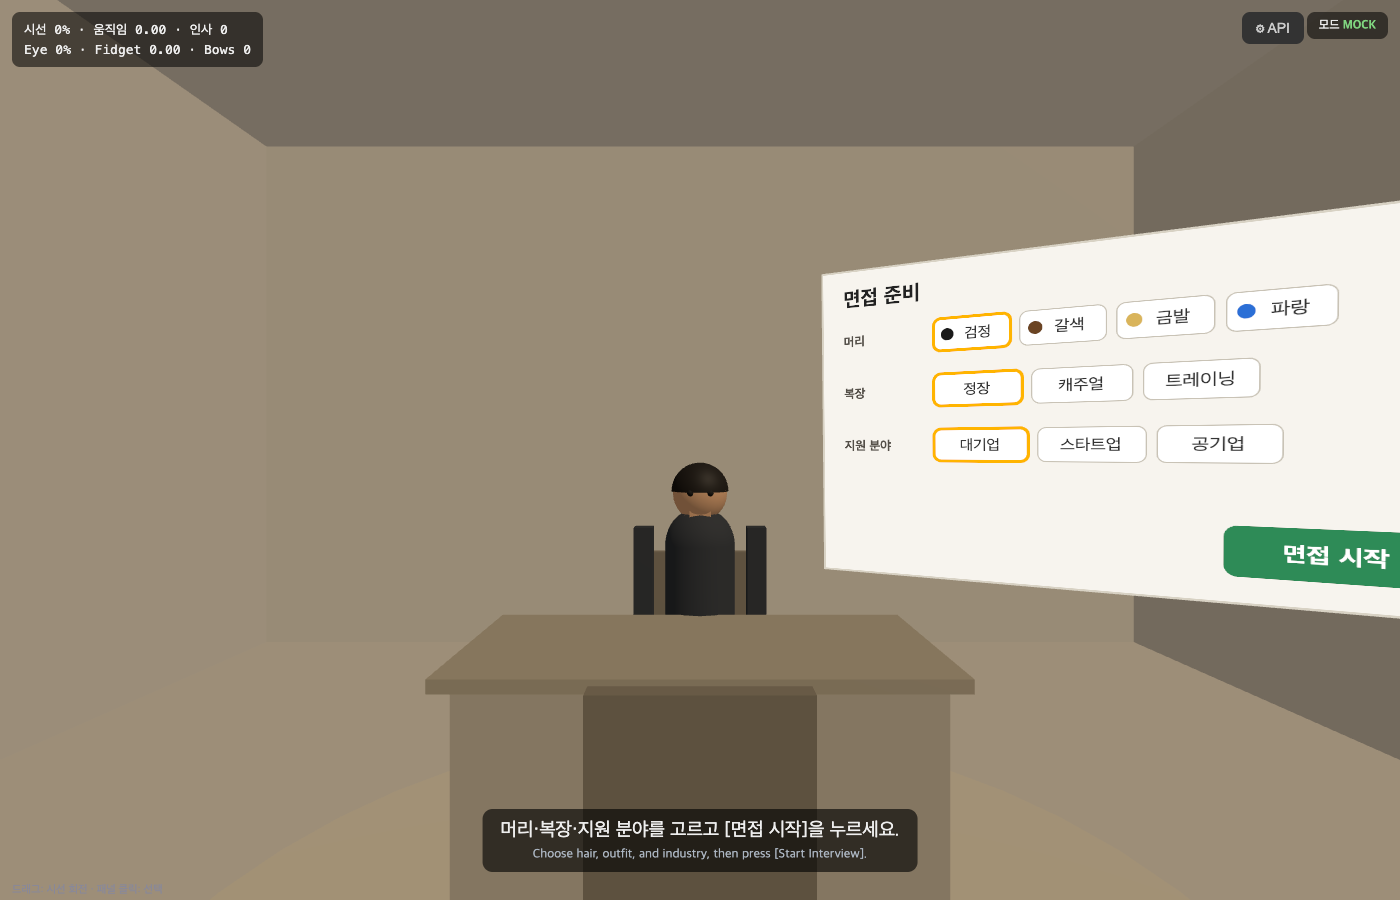
\includegraphics[width=0.44\linewidth]{dressing_room.png}\hfill
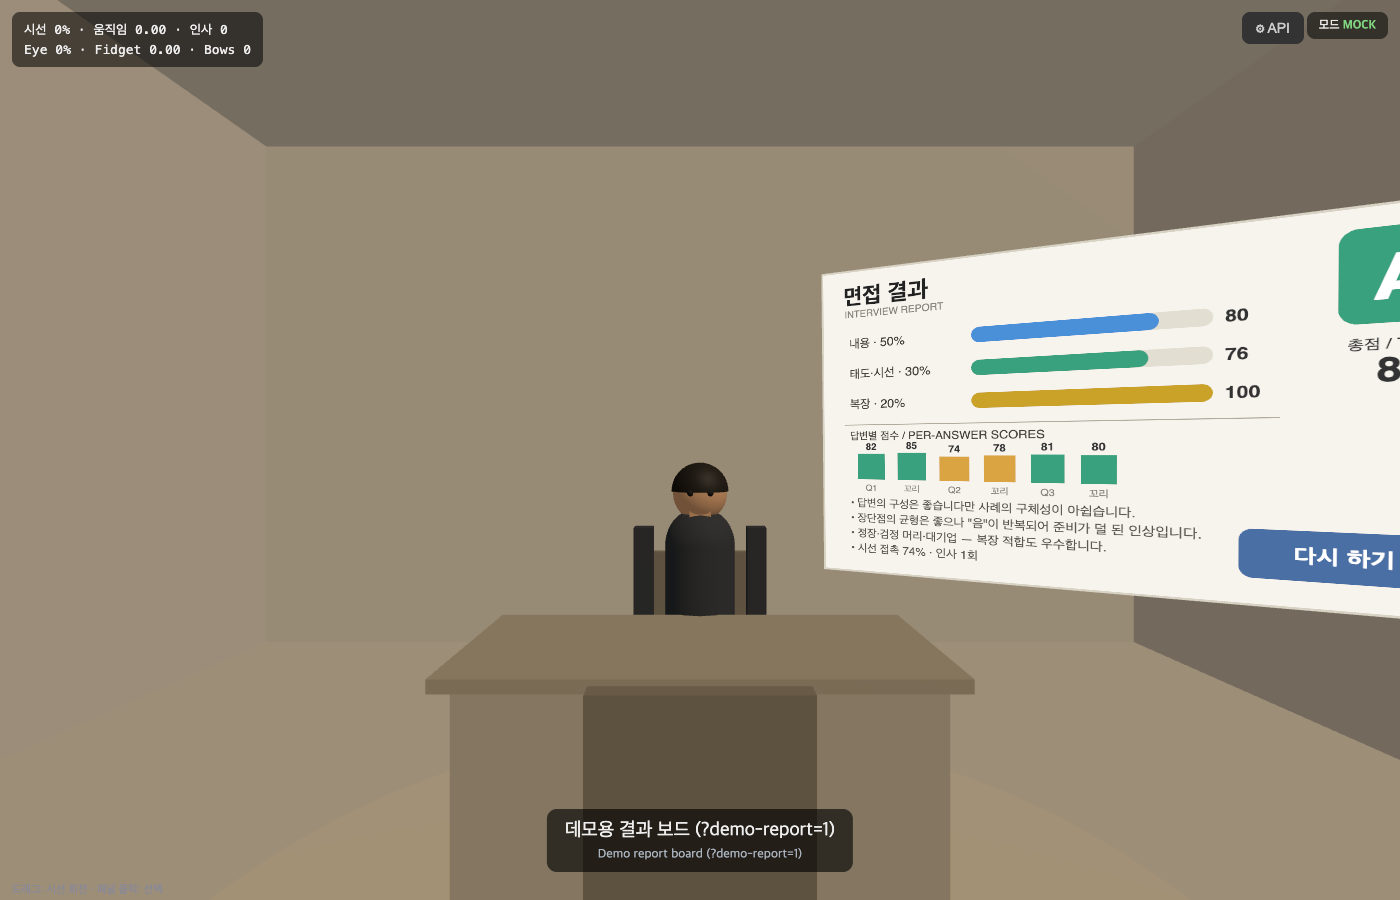
\includegraphics[width=0.44\linewidth]{report_board.png}
\captionof{figure}{Stage-1 demo run in mock mode. Left: dressing room (F1) --- selection panel and avatar at the fake mirror. Right: report board (F5) --- color-coded category bars, per-answer score chart, weighted total, and grade badge.}
\label{fig:demo}
\end{center}

\subsection{Formula spot checks}
The three binding attire examples were verified by hand arithmetic: $70{+}20{+}10=100$, $70{+}5{+}5=80$, $70{-}15{-}15=40$ (Table~\ref{tab:attire-ex}). The body-language and total formulas were verified with the worked examples of Sections 4.2 and 4.3 ($77$ and $83.1 \rightarrow$ A).

\subsection{Fallback drill}
Live mode was started with an intentionally invalid API key. Each failing call---STT, evaluation, follow-up, attire, TTS---fell back to the mock implementation for that call, and the session still completed end to end. The never-hard-fail policy held.

\subsection{Demo video}
A 3:00 screen recording was produced on macOS (Cmd+Shift+5) following the shot list in \texttt{docs/video\_script.md}: intro with motivation (0:00--0:18), dressing room (0:18--0:45), full Q1 cycle with visible HUD and greeting bow (0:45--1:52, Q2/Q3 removed by jump cut), report-board walkthrough (1:52--2:32), and architecture slide with closing (2:32--3:00). Recording in mock mode guarantees the video cannot be blocked by network or API issues.

\section{Limitations and Stage-2 Roadmap}
\textbf{Honest status.} The app was developed and verified on the macOS desktop simulator (Chrome with mouse-drag look). The Quest~2 deployment path is implemented via WebXR (own session button, \texttt{immersive-vr}, \texttt{local-floor}), but an on-device test is \emph{pending}: the team had no headset access during stage~1.

\textbf{Limitations.}
\begin{itemize}[leftmargin=1.6em,itemsep=1pt]
  \item Characters are primitive meshes; the interviewer's jaw bob is an animation, not phoneme-level lip-sync.
  \item Body language uses head pose only (camera/HMD); hands and body posture are not tracked.
  \item Three fixed questions with one follow-up each; mock-mode content is canned.
  \item Live mode stores the API key in browser \texttt{localStorage} and calls OpenAI directly from the client---acceptable for a demo, not for production.
  \item Attire vision evaluation uses an avatar screenshot, not a camera image of the user.
\end{itemize}

\textbf{Stage-2 roadmap.} Unity port (the competition's ``typical'' stack); on-device Quest~2 verification; hand tracking; real lip-sync; multi-interviewer panel; and a backend proxy for API keys.

\end{document}
